\section{Bartek Jucha}
\label{sec:bartekjucha}
\begin{figure}[h]
    \centering
    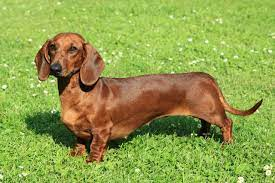
\includegraphics{pictures/jamnik.jpg}
    \caption{To jest Jamnik}
    \label{fig:jamnik}
\end{figure}



\textbf{Przykładowa maceirz 3x3:}
\begin{table}[h]
\centering
\begin{tabular}{|l|l|l|}
\hline
23 & -3 & 75 \\ \hline
21 & 43 & 1  \\ \hline
-3 & 5  & 0  \\ \hline
\end{tabular}
\end{table}



\textbf{Numeracja sportów:}
\begin{enumerate}
    \item piłka nożna
    \item siatkówka
    \item koszykówka
\end{enumerate}

\textbf{Miasta w Polsce:}
\begin{itemize}
    \item Kraków
    \item Warszawa
    \item Rzeszów
\end{itemize}



\textbf{Przykładowe wyrażenie matematyczne:}
\[f(A)^-1=\{x\in X:f(x)\in A\}\]

\newpage \textbf{Jamnik}  to rasa kiedyś wykorzystywana do polowań. Obecnie jednak psy te kojarzą się z przytulnymi psami domowymi. Mają \underline{krótkie} łapki i charakterystyczny \textit{\textbf{wydłużony tułów}} (patrz zdjecie \ref{fig:jamnik}). Ich cechy to silny charakter, żywiołowość i inteligencja. \par
Przy wyborze psa do domu czy mieszkania wiele osób decyduje się na jamnika. Ten niewielki piesek o wydłużonej, charakterystycznej budowie ciała łatwo przystosowuje się do życia w rodzinie i socjalizuje się. Możesz wybrać jamnika \textit{krótkowłosego}, \textit{szorstkowłosego} lub \textcolor{red}{długowłosego}.